\documentclass[conference]{IEEEtran}

\usepackage[bahasa]{babel}
\usepackage{cite}
\usepackage{graphicx}
\begin{document}
	\title{Metode Pengaliran Data Audio melalui Sistem Penyeimbang Muat berbasis HAProxy}
	\author{\IEEEauthorblockN{Bahrul Halimi\IEEEauthorrefmark{1},
			Putu Wiramaswara Widya\IEEEauthorrefmark{2}}
		\IEEEauthorblockA{Fakultas Teknologi Informasi,
			Institut Teknologi Sepuluh Nopember\\
			Surabaya\\
			Email: \IEEEauthorrefmark{1}bahrul.halimi11@mhs.if.its.ac.id,
			\IEEEauthorrefmark{2}wiramaswara11@mhs.if.its.ac.id}}
	
	\maketitle
	\begin{abstract}
		We propose ...
	\end{abstract}
	\begin{IEEEkeywords}
		\textit{Streaming}, HAProxy, Icecast, Penyeimbang Muat, Internet Radio.
	\end{IEEEkeywords}
	
	

	\section{Pendahuluan}
	Informasi menyebar dari lokasi ke lokasi lain dengan media yang beragam. Mulai dari media udara (percakapan) hingga media internet. Media internet inilah yang semakin meningkat tajam penggunaannya setiap tahun.
	
	\indent
	Salah satu media penyebaran informasi melalui internet adalah dengan \textit{streaming}. \textit{Streaming} sendiri sudah dikenal masyarakat Indonesia sejak lama, pada dasarnya \textit{streaming} diartikan dengan melihat video langsung dari internet tanpa harus mengunduhnya dari internet. Padahal \textit{streaming} tidak hanya menonton video saja, tapi dengan mendengarkan suara saja yang berada tidak pada lokal komputer (dari internet) bisa diartikan sebagai \textit{streaming}.
	
	\indent
	Murahnya penggunaan internet memunculkan banyaknya pelaku \textit{streaming}, baik pengguna maupun penyedia layanan. Tapi banyaknya pelaku \textit{streaming} ini tidak dibarengi dengan adanya satu gerbang yang bisa menampung beberapa penyedia \textit{streaming} dengan layanan yang cepat jika diakses oleh banyak penggunanya.
	
	\indent
	Diluar konteks \textit{streaming} persebaran informasi dalam bentuk tulisan terkadang membuat pengguna menjadi malas membukanya. Alternatif menggunakan video mulai dilirik namun kelamahannya ada pada besarnya data yang diterima pendengar sehingga terkadang dengan koneksi yang lambat juga akan memperlambat tersampainya informasi.
	
	\indent
	\textit{Audio streaming} menjadi pilihan terakhir penyampaian informasi ke pengguna. Internet radio salah satu bentuk dari \textit{audio streaming} ini. Namun, pemilik \textit{audio streaming} harus mengembangkan teknologinya sendiri untuk bisa melakukan siaran terhadap \textit{audio streaming}-nya. Walaupun aplikasi untuk melakukan \textit{streaming} ini bebas digunakan, namun dengan banyak pertimbangan (perangkat keras) akhirnya banyak yang menolak mengembangkan teknologi ini.
	
	\indent
	Metode penyeimbang muat untuk setiap permintaan yang masuk menjadi salah satu solusi dari banyaknya pengguna yang ingin menggunakan layanan audio streaming ini. Uji coba dilakukan dengan 3 node penyedia layanan yang secara bergantian melayani pengguna yang meminta layanan audio streaming. Metode penyeimbang muat memanfaatkan algoritma \textit{leastconn} yang mengambil node dengan jumlah koneksi paling sedikit.
	
	\indent
	Tulisan ini dibagi menjadi 5 (lima) bagian. Latar belakang permasalahan dijelaskan pada bagian 1. Metode penyeimbang muat dijelaskan pada bagian 2. Pada bagian 3 dan 4 akan dijelaskan skenario uji coba dan hasil uji coba. Pada akhir tulisan diuraikan kesimpulan yang diambil dari metode yang digunakan.
	
	
	\section{Metode Penyeimbang Muat}
	Audio streaming memperjelas akan adanya aliran data berupa audio yang ditransmisikan dari satu tempat ke tempat lain. Ada banyak aplikasi yang dapat mendukung aliran data audio ini sehingga tersampaikan secara utuh tanpa ada banyak noise (gangguan). Salah satu yang digunakan adalah Icecast. Dan teknologi yang dipakai untuk melakukan penyeimbang muat adalah HAProxy. Di sisi lain, metode pengaliran data audio ke beberapa node secara bersamaan akan diatur dengan nodejs.
	
	\subsection{Icecast}
	Merupakan media server streaming yang mendukung format Ogg, Opus, WebM, dan MP3. Dapat digunakan untuk membangun sebuah internet radio. Aplikasi ini berada di bawah lisensi GNU GPL. \textit{Platform} yang didukung aplikasi ini antara lain Linux, FreeBSD, OpenBSD, Solaris, dan Windows Vista hingga Windows 8 serta Windows Server 2003 hingga Windows Server 2012.
	
	\indent
	Icecast memiliki halaman administrator berupa halaman web dengan alamat 'http://ip:port'. Port dan IP yang digunakan oleh icecast sesuai dengan apa yang sudah dikonfigurasikan di dalam file icecast.xml (lokasi file biasanya ada di /etc/icecast2 untuk pengguna platform Linux).
	
	\indent
	Aplikasi ini memiliki istilah source untuk pengguna yang melakukan audio streaming. Pengguna source ini harus menentukan mount point yang digunakannya saat menggunakan aplikasi. Setiap pengguna source yang sudah melakukan stream ke server dengan mount point tertentu, layanan stream dapat didengarkan pada 'http://ip:port/mount-point-pilihan-source'. Perlu diingat IP dan port disesuaikan dengan konfigurasi sebelumnya.
	
	\indent
	Ketika melakukan stream ke alamat server dengan port yang sudah ditentukan, paket data yang dikirimkan hanya berupa paket TCP tanpa ada tambahan informasi berarti seperti pada Gambar~\ref{fig:tcp}. Paket ini membawa kelemahan dalam penyeimbangan muatan pada server utama nantinya.
	
	\begin{figure}
	\centering
	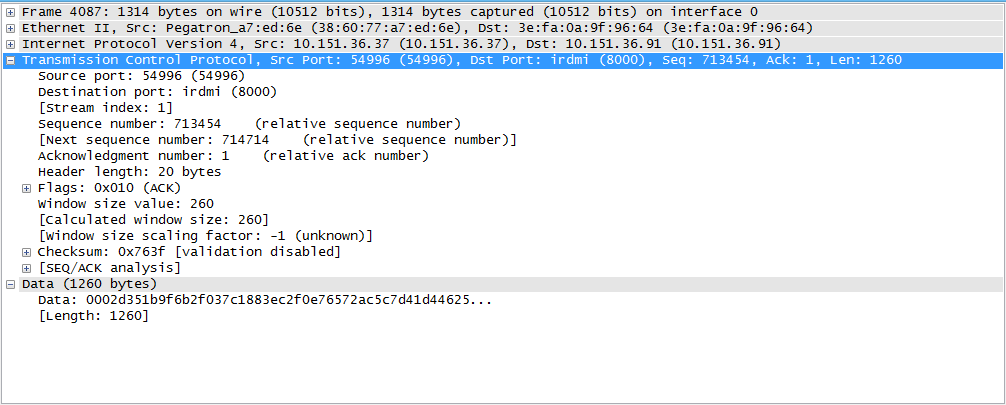
\includegraphics[width=1\linewidth]{tcp}
	\caption{Paket TCP yang dikirim streamer ke server}
	\label{fig:tcp}
	\end{figure}
	
	
	\subsection{HAProxy}
	HAProxy ( High Availability Proxy ) merupakan salah satu penyeimbang muat handal pada protokol TCP/HTTP. Sistem yang digunakannya akan membagi beban kerja ke sekumpulan server untuk memaksimalkan kerjanya. (HAProxy perlu cite
	
	\indent
	Beberapa alasan mengapa HAProxy ini banyak digunakan adalah :
	\begin{enumerate}
		\item Sangat cepat.
		\item Efisien, dengan 700 permintaan dalam satu detik CPU yang digunakan kurang dari 5\% dan 40MB RAM.
		\item Memungkinkan untuk dilakukan perubahan konfigurasi selama koneksi masih terjadi dan tidak akan mengganggu koneksi tersebut.
		\item Memungkinkan adanya queue dalam pengaplikasiannya jika memang koneksi yang masuk terlalu banyak. (Imbriaco, 2008 perlu cite
	\end{enumerate}
	
	
	\subsection{NodeJS}
	Permasalahan yang ada di dalam icecast ketika menggunakan 3 (tiga) server atau lebih secara bersamaan untuk melayani satu pengguna akan diselesaikan dengan bantuan nodejs. Streamer hanya akan mengakses satu alamat saja dan nodejs akan mengirimkan apa yang dikirimkan oleh streamer ke 3 server di alamat berbeda yang disediakan untuk melayani pengguna.
	
	\indent
	Dengan menggunakan fungsi pipe yang ada di nodejs paket TCP yang diterima satu server akan diteruskan ke 3 server lain sehingga data yang dimiliki di 3 server akan sama. Fungsi ini berada di dalam API stream. API ini sangat membantu dalam penyampaian data stream.
	
	\subsection{Penyeimbang Muat}
	
	\begin{figure}
		\centering
		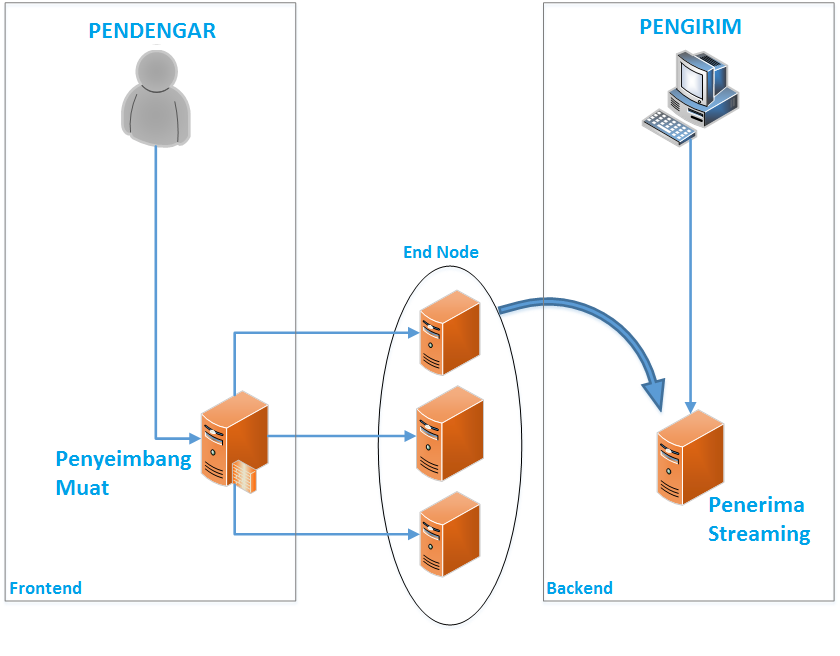
\includegraphics[width=0.7\linewidth]{arsitektur}
		\caption{Arsitektur Jaringan}
		\label{fig:arsitektur}
	\end{figure}
	
	3 (tiga) server digunakan sebagai node terakhir yang nantinya akan melayani setiap permintaan dari pengguna, dalam hal ini pengguna adalah pendengar streaming. Sementara untuk pengirim streaming disebut streamer. 
	
	\indent
	Streamer akan mengakses satu alamat server di belakang layar yang berguna untuk menerima stream. Stream ini akan diteruskan ke 3(tiga) node akhir dengan bantuan nodejs dengan metode yang sudah dijelaskan sebelumnya. Pada akhirnya ketiga node akan memiliki data stream yang sama pada waktu yang bersamaan.
	
	\indent
	Sedangkan untuk pendengar, disediakan satu alamat server penyeimbang muat (HAProxy) yang akan melayani pendengar dengan algoritma \textit{leastconn}. HAProxy memilih \textit{node} mana yang dapat melayani pendengar sesuai dengan algoritma yang sudah ditentukan. 
	
	\indent
	Arsitektur jaringan secara utuh sesuai dengan Gambar~\ref{fig:arsitektur}. Sehingga nantinya akan terdapat dua bagian utama yaitu frontend yang berhadapan langsung dengan pendengar dan backend yang hanya berurusan dengan \textit{streamer}. Hanya saja ketika streamer menginginkan akses baru ke dalam server, \textit{streamer} harus mendaftarkan dirinya sebagai pengguna sah server.
	
	

	

	
	\section{Skenario Uji Coba}
	
	\section{Hasil Uji Coba}
	
	\section{Kesimpulan}
	
	\section{Daftar Pustaka}

\end{document}